% !Mode:: "TeX:UTF-8"

\chapter{实验设计与分析}
\label{ch:exp}

本章将利用社会关系理解的数据集对上一章提到的PPRN模型进行社会关系图谱生成的验证,具体来说即识别出图片中两个标定坐标人之间的关系类别。本章首先介绍当前所用到的两个数据集中训练/验证/测试集的数据分布情况,数据集的特点。再介绍若干对比模型,介绍实验的参数设置,然后分别对实验结果进行说明和分析,并且对其中消息池化进行了不同实现方法的对比。最后通过案例研究的方法来具体分析PPRN模型在社会关系图谱生成中发挥的效果。

\section{数据集}

\subsection{数据集简介}

现有大规模社会关系理解的数据集主要有两个:分别是PIPA-relation\cite{sun2017a}数据集和PISC\cite{li2017dual-glance}数据集,下面简单介绍这两个数据集。
PISC数据集全称是People in social Context,它是Sun等人\cite{sun2017a}在2017年通过人工标注平台得到的数据集,这些图片主要来自Visual Genome\cite{krishna2017visual}、COCO\cite{lin2014microsoft}、YFCC100M\cite{thomee2016yfcc100m:}、instagram 和twitter等社交网站、Google和Bing商业搜索引擎。数据的来源可以保证数据集的图片有足够高的方差,足够数量人的面部表情,以及场景类型。PISC数据集包含22670张图片以及对应的社会关系标注,在PISC数据集上,又包含两个粒度的识别任务,coarse-level和fine-level。如图\ref{fig:exp-pisc-r}所示的划分方式,先是粗粒度的,再到细粒度的关系类别。
\begin{figure}[htpb]
	\centering
	%	\includegraphics[width=0.48 \textwidth, trim=10 10 10 80,clip]{./pic/example_new.pdf}
	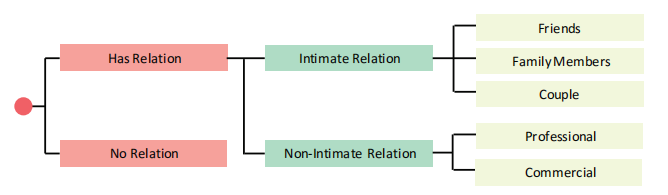
\includegraphics[width=0.98 \textwidth,clip]{pisc-split.png}
	%\hspace{0.02\textwidth}
	%\vspace*{-0.08cm}
    \caption{PISC\cite{li2017dual-glance}的关系划分}
	\vspace*{-3.5mm}
	\label{fig:exp-pisc-r}
\end{figure}

PIPA-relation数据集的全称是People in Photo Album Relation,总共包括37107张图片。同样是人工标注的数据集,基于社会关系理论划分的,Sun\cite{sun2017a}详细的给出了每个关系域的特征。然后所有的社会关系划分为5个关系域,在构建数据集的过程中,这5个关系域划分为16种社会关系,五个关系域分别是Attachment domain、Reciprocity domain、Mating domain、Hierarchical power domain和Coalitional groups domain。Attach domain划分为{\it father-child},{\it mother-child},{\it Grandpa-grandchild}和{\it grandma-grandchild},Reciprocity domain划分为{\it friends}, {\it siblings}和{\it classmates}。Mating domain 只包含单条关系{\it lovers/spouses}。Hierarchical power domain划分为{\it presenter-audience}, {\it teacher-student}, {\it trainer-trainee}和 {\it leader-subordinate}。Coalitional groups domain划分为{\it band members}, {\it dance team members}, {\it sport team members} 和 {\it colleagues} 。

数据集的情况如表\ref{tab:exp-sta-one},``Train''表示训练集图片的数量,``Valid''和``Test''分别表示验证和测试集的图片数量。``\#train''表示训练集人对的数量,``\#valid''和``\#test''分别表示验证和测试集的人对数量。
\begin{table}[htpb]
  \centering
  \caption{PISC、PIPA-relation数据集的统计表1}
  \label{tab:exp-sta-one}
  \setlength{\tabcolsep}{4.5mm}
  \begin{tabular}{c|c|c|c|c|c|c}
    \toprule
    数据集 & Train & Valid & Test & \#train  &  \#valid &  \#test  \\
    \midrule
    PISC-coarse & 13142 & 4000 & 4000 & 14536 & 2
    36 & 15497   \\
    \midrule
    PISC-fine &  16828 & 500 & 1250 & 55400 & 1505 & 3691 \\
    \midrule
    PIPA-relation & 5857 & 261 & 2452 & 13729 & 709 & 5106 \\
    \bottomrule
  \end{tabular}
\end{table}

\subsection{数据集分析} \label{sec:exp-dataset-ana}

对于数据集PISC-coarse、PISC-fine和PIPA-relation,本文做了基本的数据集分析,如表\ref{tab:exp-sta-two},其中``Sui''表示一张图片有多个人对的比例,``Unsui''则表示一张图片只有一个人对的百分比。``Single Rel''一张图片包含的关系类别只有一种,``Multi Rel''表示一张图片包含多种关系。从表统计数据可以得到两个结论,从``Sui''和``Unsui''来看,绝大多数的图片是包含多个人对的,从``Multi Rel''来看,一张图片的关系种类往往是相同的,同时直观来看,给定场景下的社会关系是稳定的。假设一张图片是一个会议的场景,那么其中往往会有多个人对,并且这些人对间的社会关系往往是{\it colleagues}或{\it presenter audience}。
\begin{table}[htpb]
  \centering
  \caption{PISC、PIPA-relation分析表,单位为(\%)}
  \label{tab:exp-sta-two}
  \begin{tabular}{c|c|c|c|c}
    \toprule
    数据集 & Sui. & Unsui. & Single Rel & Multi Rel \\
    \midrule
    PISC-coarse  & 87.1 & 12.9 & 79.9 & 20.1 \\
    \midrule
    PISC-fine  & 83.9 & 16.1 & 86.4 & 13.6 \\
    \midrule
    PIPA-relation & 71.9 & 28.1 & 94.9 & 5.1 \\
    \bottomrule
  \end{tabular}
\end{table}

此外,对于关系类别这项统计,本文做了进一步工作,并且发现一张图片的关系种类大多只是一种,少部分是两种。如图\ref{fig:exp-statistic}所示,在PISC-coarse中,大约79.9\%的图片是只有一种关系类别,20.0\%的图片有含有两个关系。

\begin{figure}[htpb]
	\centering
	%	\includegraphics[width=0.48 \textwidth, trim=10 10 10 80,clip]{./pic/example_new.pdf}
	\subfigure[pisc-coarse]{
    	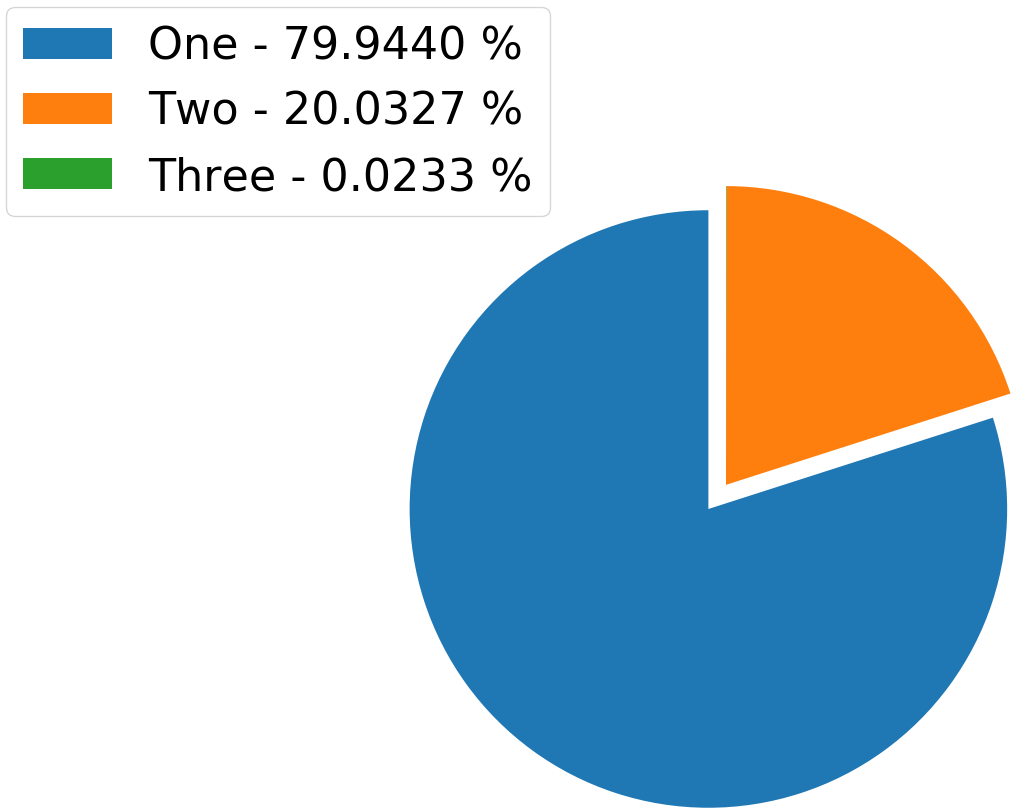
\includegraphics[width=0.30 \textwidth,clip]{PISC_coarse.png}
    	%\hspace{0.02\textwidth}
    	%\vspace*{-0.08cm}
        %\caption{数据集的关系类别统计}
    	\vspace*{-2.5mm}
    }
    \subfigure[pisc-fine]{
    	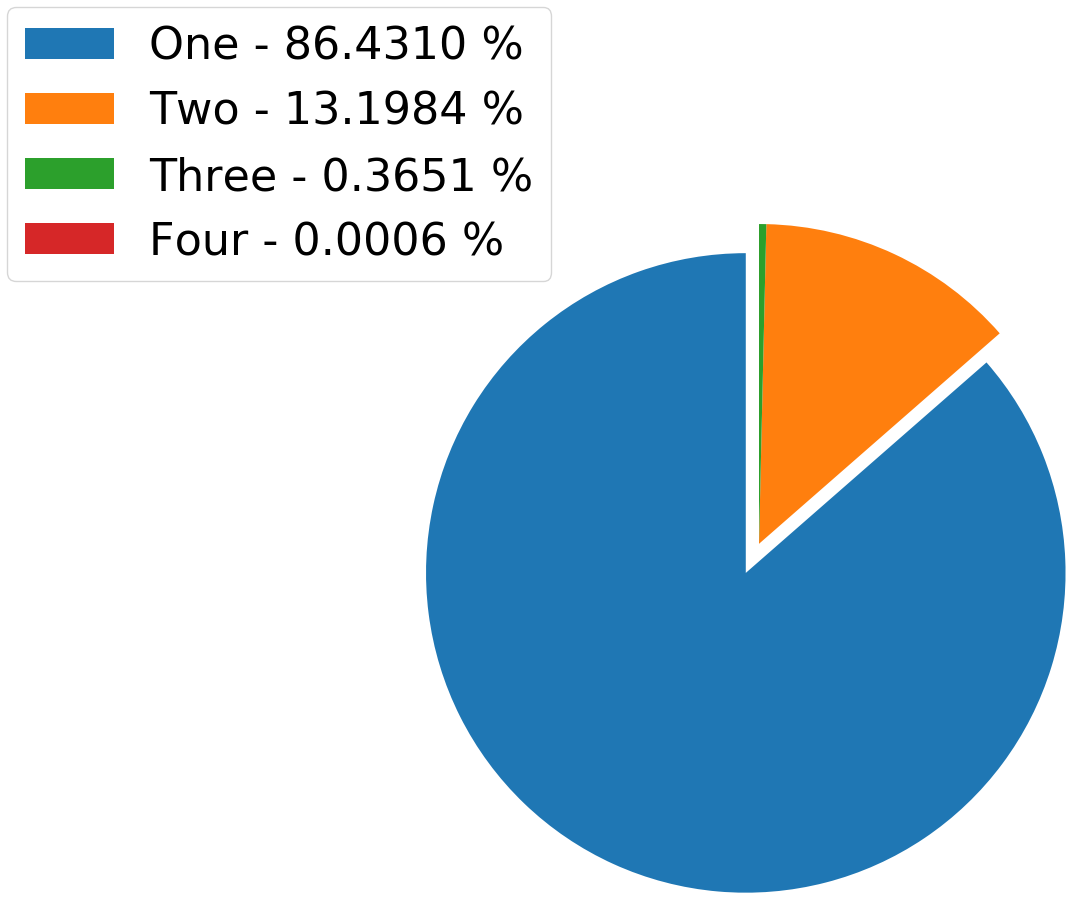
\includegraphics[width=0.30 \textwidth,clip]{PISC_fine.png}
    	%\hspace{0.02\textwidth}
    	%\vspace*{-0.08cm}
        %\caption{数据集的关系类别统计}
    	\vspace*{-2.5mm}
    }
    \subfigure[pipa-relation]{
    	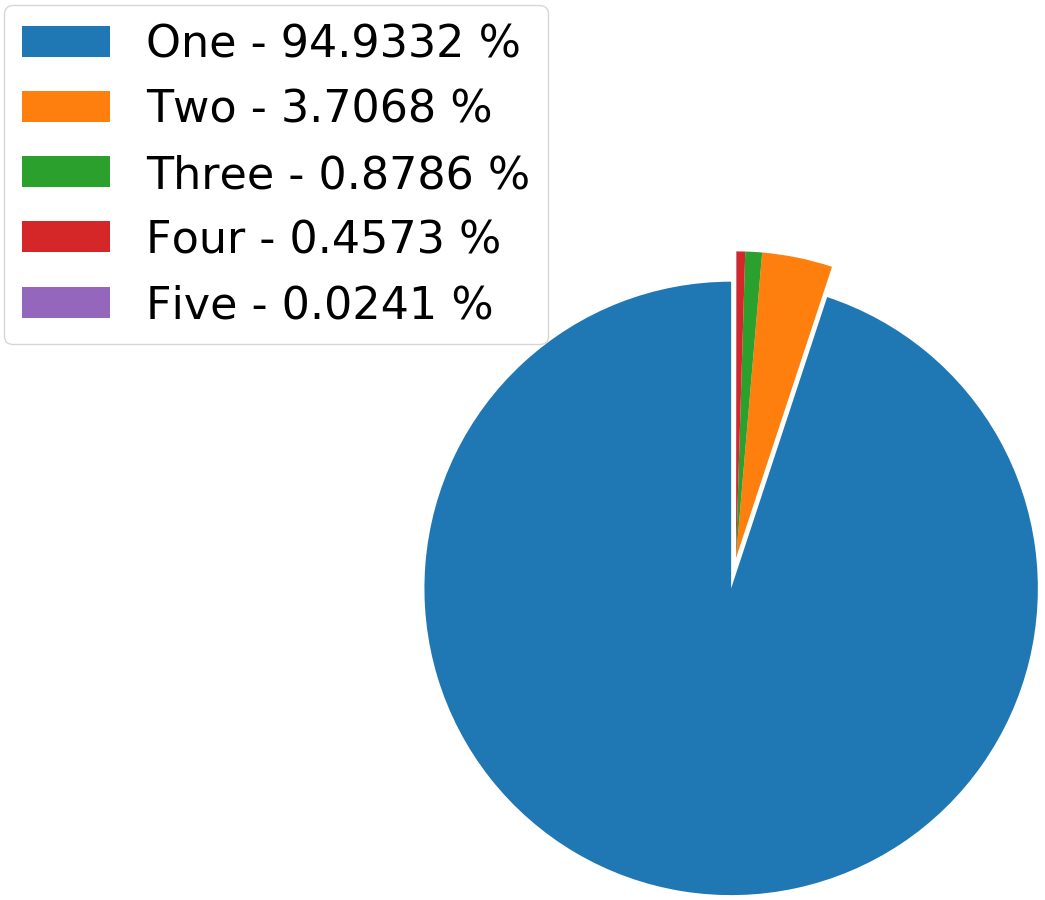
\includegraphics[width=0.30 \textwidth,clip]{PIPA_fine.png}
    	%\hspace{0.02\textwidth}
    	%\vspace*{-0.08cm}
        %\caption{数据集的关系类别统计}
    	\vspace*{-2.5mm}
    }
    \caption{数据集的关系类别统计}
	\vspace*{-3.5mm}
	\label{fig:exp-statistic}
\end{figure}

\section{实验设置}

类似于GRM模型,我们采用的是每个类别的召回率和mAP(mean average precision)。mAP常作为物体检测任务的评价标准,它是不同召回值下最大精度的平均值。举例如下,假设当前图片有五个苹果,首先对物体检测模型所有检测框分类的类别为苹果按得分从大到小排序。依次计算准确率和召回率,这里的准确率指的是TP和FP。 假如总共有10个检测框被识别为苹果,其计算结果如表\ref{tab:exp-map}所示,例如其中的对于排名第三的样本,$\textbf{Precision} = 2/3 = 0.67$,$\textbf{Recall} = 2/5 = 0.4$。
\begin{table}[htpb]
  \centering
  \caption{mAP计算示例数据}
  \label{tab:exp-map}
  \begin{tabular}{c|c|c|c|c|c|c|c}
    \toprule
    \textbf{得分排名} & \textbf{correct?} & \textbf{Precision} & \textbf{Recall}  & \textbf{得分排名} & \textbf{correct?} & \textbf{Precision} & \textbf{Recall}   \\
    \midrule
    1 & True & 1.0 & 0.2  & 6 & True & 0.5 & 0.6    \\
    \midrule
    2 &  True & 1.0 & 0.4  & 7 & True & 0.57 & 0.8  \\
    \midrule
    3 & False & 0.67 & 0.4  & 8 & False & 0.5 & 0.8  \\
    \midrule
    4 & False & 0.5 & 0.4   & 9 & False & 0.44 & 0.8 \\
    \midrule
    5 & False & 0.4 & 0.4  & 10 & True & 0.5 & 1.0 \\
    \bottomrule
  \end{tabular}
\end{table}
根据数据,以Recall为横坐标,Precision为纵坐标,可以画出如图\ref{fig:exp-map}所示的曲线B。将recall 值划分为11个值,我们将$Recall \geq \widetilde{r}$的Precision 替换为最大的,由此可得到曲线C。计算方法如公式
\ref{eq:exp-map}所示。我们给定的数据,对于苹果这一类别的AP = $(5 \times 1.0 + 4 \times 0.57 + 2 \times 0.5)/11$
\begin{figure}[htpb]
	\centering
	%	\includegraphics[width=0.48 \textwidth, trim=10 10 10 80,clip]{./pic/example_new.pdf}
	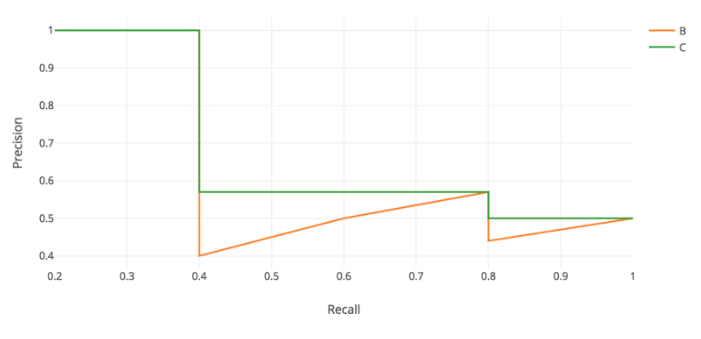
\includegraphics[width=0.75 \textwidth,clip]{map.png}
	%\hspace{0.02\textwidth}
	%\vspace*{-0.08cm}
    \caption{mAP计算示例图}
	\vspace*{-3.5mm}
	\label{fig:exp-map}
\end{figure}
\begin{equation} \label{eq:exp-map}
\begin{split}
    \mathbf{AP} = \frac{1}{11}\sum_{r \in \{0.0,0.1....,1.0\}}P_{interp}(r) \\
    \mathbf{P}_{intern}(r) = max_{\widetilde{r} \geq r}p(\widetilde{r})
\end{split}
\end{equation}

对于本文使用的预训练模型,包括ResNet-101和Vgg-16最后一层的维度都是是4096,经过全连接层,在消息传递和池化模块的中的编码长度为512。结合周边物体信息模块中注意力机制的attention\_size=30。对于RPN网络的检测框,我们设定取得分最高的30个检测框。在微调ResNet-101和Vgg-16网络时,卷积层学习率设置为$1 \times 10^{-4}$,针对任务设定的分类层学习率为$1 \times 10^{-3}$。训练时,学习率设置为$1 \times 10^{-4}$,权重衰减为$5 \times 10^{-4}$。对于PISC-coarse和PISC-fine数据集,消息传递和池化模块的迭代数$T=4$,PIPA-relation数据集,迭代次数为$T=3$。 微调时的优化方法是SGD,训练迭代模块的优化方法是Adam。

\section{PISC数据集实验结果}
在实验中,本文主要与以下几个模型进行对照,在我们的整体框架中,主要有特征提取模块(m0)、消息传递和池化模块(m1),关系和关系域损失(m2)、周边物体信息模块(m3)。对于m0和m1组成的网络为PPRN,而m0、m1、m2三个模块一起的模型称为PPRN+d,所有模块的模型简称为PPRN+d+obj:
\begin{itemize}
    \item \textbf{Union CNN}学习Lu等人\cite{lu2016visual}利用一个CNN网络来预测关系方法,同样利用一个CNN网络来提取人对的联合区域的特征来进行分类任务。
    \item \textbf{Pair CNN}\cite{li2017dual-glance}由两个共享参数的CNNs提取两个修剪出来的图像特征进行分类。
    \item \textbf{Pair CNN + BBox + Union}\cite{li2017dual-glance}在前面两个特征提取模块的基础上,进一步结合两个个体包围盒的联合区域特征和包围盒的位置特征。
    \item \textbf{Dual-glance}\cite{li2017dual-glance}实现两个粒度的分类任务,分别是PISC-coarse 和PISC-fine,分别包含3种和6种关系类别。Dual-glance利用了PairCNN+BBox+Union,以及物体区域的特征来提纯预测结果。
    \item \textbf{GRM}\cite{wang2018deep}提出了一个图推理模型来提升社会关系理解任务,该模型集成物体和社会关系共现概率的先验知识,GRM采用的是人对特征和上下文物体特征之间的消息传递。
\end{itemize}

在表\ref{tab:exp-result-1}中,我们展示了在PISC数据集上,按照每个类别的召回率和``mAP''的设定得到的实验结果,这里需要说明,因为在PISC-coarse中的关系粒度已经是最粗的,所以在实际实现过程中只存在关系损失,domain loss只在PISC-fine 和PIPA 数据集上进行了实验。
\begin{table*}[htpb]
  \centering
  \caption{在PISC-coarse上的实验结果,单位为百分比(\%)}
  \label{tab:exp-result-1}
  \begin{tabular}{c|c|c|c|c}
    \toprule
    模型 & Intimate & Non-Intimate & No Relation & mAP  \\
    \midrule
    Union CNN \cite{lu2016visual} & 72.1 & 81.8 & 19.2 & 58.4   \\
    \midrule
    Pair CNN \cite{li2017dual-glance}  & 70.3 & 80.5 & 38.8 & 65.1   \\
    \midrule
    Pair CNN + BBox + Union \cite{li2017dual-glance}  & 71.1 & 81.2 & 57.9 & 72.2   \\
    \midrule
    Pair CNN + BBox + Global \cite{li2017dual-glance}  & 70.5 & 80.0 & 53.7 & 70.5  \\
    \midrule
    Dual-glance \cite{li2017dual-glance} & 73.1 & \textbf{84.2} & 59.6 & 79.7  \\
    \midrule
    GRM \cite{wang2018deep} & 81.7 & 73.4 & 65.5 & \textbf{82.8}   \\
    \midrule
    PPRN & \textbf{81.9} & 67.3 & \textbf{74.7} & 81.8  \\
    \midrule
  \end{tabular}
\end{table*}

与此同时,在表\ref{tab:exp-result-2}中,我们也展示了在PISC-fine数据集上,同样按照mAP的设定之后得到的实验结果。
\begin{table*}[htpb]
  \centering
  \caption{在PISC-fine上的实验结果,单位为百分比(\%)}
  \label{tab:exp-result-2}
  \begin{tabular}{c|p{1.5cm}<{\centering}|p{0.8cm}<{\centering}|p{0.8cm}<{\centering}|p{0.8cm}<{\centering}|p{0.8cm}<{\centering}|p{0.8cm}<{\centering}|c}
    \toprule
     模型& \rotatebox[origin=l]{90}{Friends} & \rotatebox[origin=l]{90}{Family} & \rotatebox[origin=l]{90}{Couple} & \rotatebox[origin=l]{90}{Professional} & \rotatebox[origin=l]{90}{Commercial} & \rotatebox[origin=l]{90}{No Relation} &  \rotatebox[origin=l]{90}{mAP}  \\
    \midrule
    Union CNN  \cite{lu2016visual} & 29.9 & 58.5 & 70.7 & 55.4 & 43.0 & 19.6 & 43.5  \\
    \midrule
    Pair CNN \cite{li2017dual-glance} & 30.2 & 59.1 & 69.4 & 57.5 & 41.9 & 34.2 & 48.2   \\
    \midrule
    Pair CNN + BBox + Union \cite{li2017dual-glance} & 32.5 & 62.1 & 73.9 & 61.4 & 46.0 & 52.1 & 56.9   \\
    \midrule
    Pair CNN + BBox + Global \cite{li2017dual-glance} & 32.2 & 61.7 & 72.6 & 60.8 & 44.3 & 51.0 & 54.6  \\
    \midrule
    Dual-glance\cite{li2017dual-glance} & 35.4 & 68.1 & 76.3 & 70.3 & 57.6 & 60.9 & 63.2  \\
    \midrule
    GRM \cite{wang2018deep} & 59.6 & 64.4 & \textbf{58.6} & 76.6 & 39.5 & 67.7 & 68.7   \\
    \midrule
    PPRN & \textbf{61.0} & 67.1 & 56.2 & \textbf{76.9} & 46.0 & 68.1 & 69.7 \\
    \midrule
    PPRN+d(PPRN+domain loss) & 58.2 & \textbf{68.9} & \textbf{74.6} & 63.3 & \textbf{67.6} & \textbf{70.3} & \textbf{72.0} \\
    \bottomrule
  \end{tabular}
\end{table*}
根据\ref{tab:exp-result-1},\ref{tab:exp-result-2}和表\ref{tab:exp-mp-variant}所示的实验结果,我们可以得出以下结论:
\begin{enumerate}
    \item 首先,Pair CNN + BBox + Global,Dual-glance和GRM都引入了额外的Faster-RCNN\cite{ren2015faster}来抽取当前图片的上下文信息(物体区域)。GRM进一步利用识别出的物体类别构建了物体类别和社会关系类别的语义共现的知识图谱,通过神经网络融入关系类别和上下文线索的先验常识知识,进而来解决社会关系理解问题。需要提到的是这些模型均引入了额外的检测标注,而这些步骤是会带来额外的噪声和性能消耗的,而PPRN不存在这些外部因素。
    \item 其次,结合表\ref{tab:exp-result-1}、表\ref{tab:exp-result-2}的实验数据,对于coarse-level的识别,PPRN取得了75.1\% 的准确率,81.8\%的mAP。对于fine-level的识别,PPRN-取得了65.7\%的准确率,69.7\% 的mAP。本文提出的模型在fine-level 的识别任务上超过了所有的基准模型。与此同时,PPRN+d(PPRN+domain loss)取得了66.2\%的准确率,72.0\%的mAP,证明了引入domain loss的作用。模型在coarse-level的识别任务上略微低于GRM,但是仍然超过了其它引入了周边物体区域的模型。
\end{enumerate}

\section{PIPA-relation数据集实验结果}

在PIPA-relation数据集上,本文和现有的方法进行了对比,例如:Two Stream CNN\cite{sun2017a},Dual-glance\cite{li2017dual-glance}和GRM\cite{wang2018deep},这些模型在之前均取得了最好识别效果。本文直接从文献中获取这些模型的实验数据,如表\ref{tab:exp-pipa-table}所示,由于有的关系的样本数量较少,所有的基准模型均只采用准确率衡量模型的效果,因此本文同样如此。值得提到的是,PPRN明显超过现有的基准模型,比GRM超过2.4\%,比Dual-glance超过5.1\%。
PPRN+d(PPRN+domain loss)取得了63.6\%识别率,高于基准模型,轻微低于不引入关系域损失的PPRN模型。
\begin{table}[htpb]
  \centering
  \caption{准确率的单位为百分比 (\%) PPRN、PPRN+d在PIPA-relation实验结果}
   \vspace*{-3.5pt}
  \label{tab:exp-pipa-table}
  \begin{tabular}{c|c}
    \toprule
    模型 & accuracy \\
    \midrule
    Two stream CNN \cite{zhang2015beyond} & 57.2 \\
    \midrule
    Dual-Glance \cite{li2017dual-glance} & 59.6 \\
    \midrule
    GRM \cite{wang2018deep} & 62.3 \\
    \midrule
    PPRN & \textbf{64.7} \\
    \midrule
    PPRN+d(PPRN+domain loss)  & 63.6 \\
    \bottomrule
  \end{tabular}
\end{table}

\section{实验结果分析}

在本文中,最核心的部分即消息传递机制的引入,其中起到核心作用的包括采用可学习的参数来聚合社会关系图谱中其它节点的隐藏层编码。同时为了进一步证明当前方法的作用,我们分别采用了其它标准的池化方法,包括average pooling、max pooling。实验结果如表\ref{tab:exp-mp-variant}所示,并且在表中给出了PPRN+d+obj在PISC数据集上的实验结果。
\begin{table}[htb]
	\vspace*{-3.5pt}
	\centering
	\caption{RCNN的mAP和准确率的实验结果,消息池化模块采用不同的方式的结果,其中PPRN(attention)即本文实现结果,所有实验数据的单位为百分比(\%)}
    \label{tab:exp-mp-variant}
	\vspace*{0.5mm}
	\begin{tabular}{c|c|c|c|c}
		\toprule
		\multirow{2}{*}{评价标准} &
		\multicolumn{2}{c|}{PISC coarse} &
		\multicolumn{2}{|c}{PISC fine}  \\
				 & accuracy & mAP & accuracy & mAP  \\
		\midrule
		RCNN & - & 63.5 & - & 48.4 \\
		\midrule
		PPRN(max pooling) & 74.3 & 80.8 & 64.1 & 68.1 \\
		\midrule
		PPRN(avg pooling) & 74.6 & 80.1 & 63.8 & 68.3 \\
		\midrule
		PPRN(attention) & \textbf{75.1} & \textbf{81.8} & \textbf{65.7} & \textbf{69.7} \\
		\midrule
		PPRN+d  & - & - & \textbf{66.2} & \textbf{72.0} \\
        \midrule
		PPRN+d+obj  & 74.9 & 81.2 & 65.3 & 69.1 \\
		\midrule
	\end{tabular}
\end{table}

根据表\ref{tab:exp-pipa-table}、表\ref{tab:exp-mp-variant}所展示的实验结果,我们可以得到以下的结论:
\begin{enumerate}
    \item 首先,对于前面提到的PPRN模型的主要工作是捕获关系之间交互的文信息,没有考虑周边的物体信息,考虑这部分的信息是需要引入额外的物体检测模型。PPRN+d+obj在消息传递机制的基础上进一步加入周边物体的信息,但是在多个实验中并没有超过未引入这部分信息的基准模型。从周边的物体信息的角度来看,周边的物体信息可以认为是形成了一个场景,物体上下文特征起作用的前提是物体检测和识别模型性能效果,同时这部分的特征形成的场景信息往往是单一的,对最后的关系编码的约束也是单一的,同时考虑关系的上下文类似于考虑上下文物体的信息。
    \item 其次,在GRM等引入关系类别和物体类别共现的常识知识,很大程度依赖物体的类别是否正确,才能确定加入的常识知识是否正确。第一,例如在当前图片中,检测到了{\it laptop},容易倾向于推理出当前场景下所有人对关系为{\it professional},但是Faster-RCNN并不是总能识别正确,所以会带来很大的噪声。第二,检测出的{\it laptop}会帮助{\it professional}关系的正确分类,但是对{\it friends}来说并不存在这样的辅助作用,并且这两类关系在现实数据集和场景中大量存在。
    \item 本文通过引入的domain loss,在PISC-fine上取得了明显的提升,模型通过同时优化relation loss和domain loss,这样两个任务之间可以共享一些信息,并且相互约束,帮助区分属于不同关系域的关系。
    \item 如表\ref{tab:exp-mp-variant}所示,RCNN是只用到了图片中物体信息,是最差的效果。Dual-glance训练了一个基于注意力机制的人对模块根据不同的人对关系来结合不同比重的物体特征。对于模型PPRN+d+obj来说,模型效果并没有提升,依据前面的分析,关系上下文覆盖了周边物体区域上下文的部分,并且实验证明了我们的假设。
    \item 就目前来看,模型在粗粒度的分类任务上并不如现有的最优模型,图片的场景信息对于判断亲密与否帮助很大。是否可以尝试挖掘更多的信息引入模型,例如年龄,性别,这部分细粒度的特征会帮助细粒度的关系分类,但是目前模型并没有这在这方面进行探索,模型的实验结果虽然由于最优模型,但是是否可以有更大的提升。
\end{enumerate}

\section{案例研究}

除此之外,为了观察PPRN在社会关系理解任务上的具体表现,我们在PISC-fine的测试集中随机抽取了部分图片,并且列出了他们的具体表现。在图\ref{fig:exp-case-study}中,我们分别展示了4个样例的结果,左边代表原图片,右边是生成的社会关系图谱,其中(A)表示标注,(B)表示我们模型构建的社会关系图谱,(C)表示基准模型中GRM的结果。其中图片中人的包围盒的颜色对应社会关系图谱中节点的颜色,节点间不同颜色的边表示不同的社会关系,在图
\ref{fig:exp-case-study}中列出了颜色和关系的对应表。从这四个例子来看,相比于GRM生成的社会关系图谱(C),(B)的准确率和mAP更高。并且这四个例子都有各共同点,(B)中每张图超过一半的人对关系都预测为是一样的,如\ref{sec:exp-dataset-ana}提到的,每张图片的场景是稳定的,每张图片包含的社会关系几乎是相似或者是一样的。因此,本文提出的模型恰好能利用上这个线索,对于第样例(a)来说,有两类关系,{\it Commercial}和
{\it No Relation}, 橘色包围盒的人和绿色包围盒的人之间的关系在GRM 中错误的预测为{\it couple},但是PPRN能正确的分类。就这张图片来说,PPRN的准确率是100\%,但是GRM是33.3\%。
\begin{figure}[htpb]
	\centering
	%	\includegraphics[width=0.48 \textwidth, trim=10 10 10 80,clip]{./pic/example_new.pdf}
	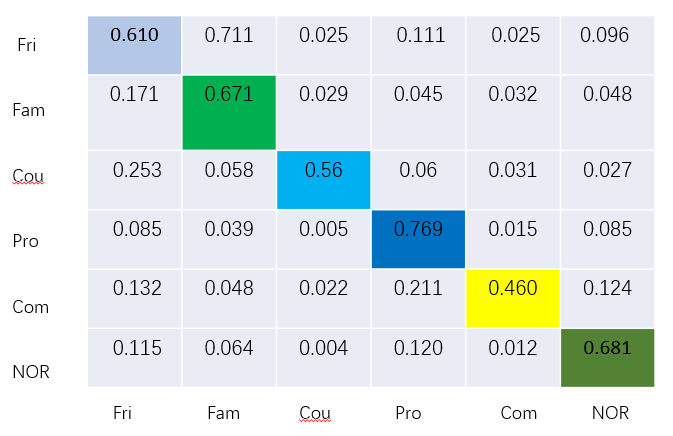
\includegraphics[width=0.75 \textwidth,clip]{confu-matrix.png}
	%\hspace{0.02\textwidth}
	%\vspace*{-0.08cm}
    \caption{PPRN模型在6种关系、fine-level数据集上的混淆矩阵结果}
	\vspace*{-3.5mm}
	\label{fig:exp-confu-fine}
\end{figure}

直观来看,{\it Friend}和{\it Commercial}很难预测,并且这也符合所有的模型来说在fine-level的识别结果。以本文提出的为例,在fine-level的召回混淆矩阵如图\ref{fig:exp-confu-fine}所示,相比其他非亲密的关系,({\it Friend},{\it Couple},{\it Family})这三种关系之间更容易相互混淆,意味着他们有相似的特征。但是,非亲密的关系({\it Professional},{\it Commercial})互相之间不存在容易混淆的情况。同理,如图
\ref{fig:exp-confu-coarse}所示,为coarse-level的混淆矩阵,{\it Intimate}容易和{\it No-relation}之间互相混淆,而{\it Non-intimate}相比{\it No-relation},更容易与{\it Intimate}混淆。
此外,图\ref{fig:exp-error-case}给出了一些错误的测例,例如第一行第一张图,模型错误的将夫妻关系分类为朋友关系。
\begin{figure}[htpb]
	\centering
	%	\includegraphics[width=0.48 \textwidth, trim=10 10 10 80,clip]{./pic/example_new.pdf}
	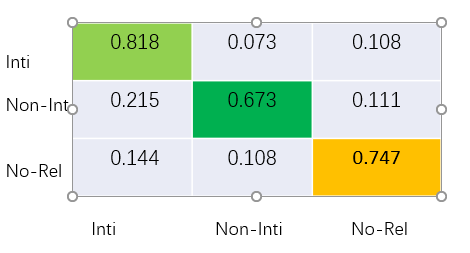
\includegraphics[width=0.55 \textwidth,clip]{coarse-confu-matrix.png}
	%\hspace{0.02\textwidth}
	%\vspace*{-0.08cm}
    \caption{PPRN模型在3种关系、coarse-level数据集上的混淆矩阵结果}
	\vspace*{-3.5mm}
	\label{fig:exp-confu-coarse}
\end{figure}

\begin{figure}[htpb]
	\centering
	%	\includegraphics[width=0.48 \textwidth, trim=10 10 10 80,clip]{./pic/example_new.pdf}
	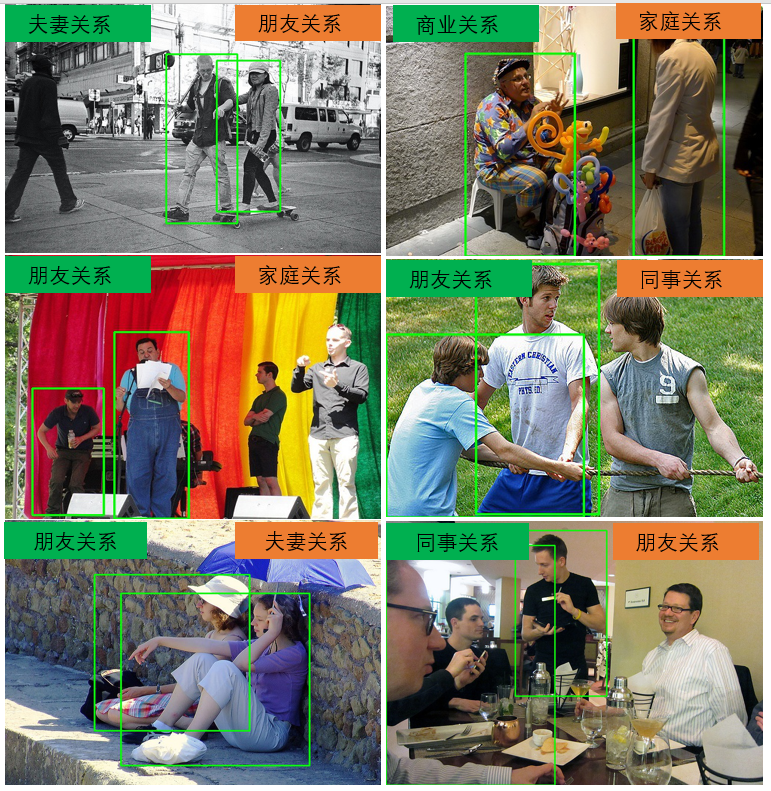
\includegraphics[width=0.75 \textwidth,clip]{case-error.png}
	%\hspace{0.02\textwidth}
	%\vspace*{-0.08cm}
    \caption{错误识别的测例,左边的标签是标注,右边的标签是模型预测结果}
	\vspace*{-3.5mm}
	\label{fig:exp-error-case}
\end{figure}

\begin{figure}[htpb]
	\centering
    \subfigure[]{
    	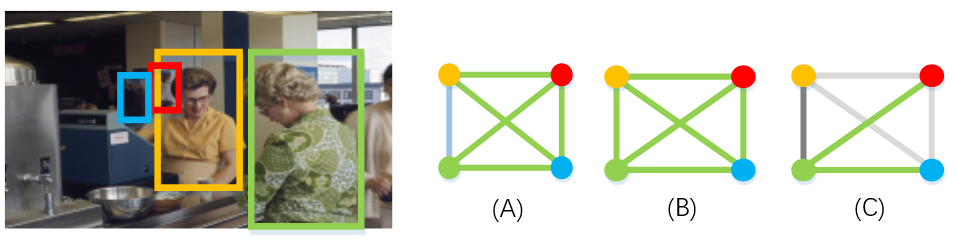
\includegraphics[width=0.90 \textwidth,clip]{case-1.png}
    	%\hspace{0.02\textwidth}
    	%\vspace*{-0.08cm}
        %\caption{数据集的关系类别统计}
    	\vspace*{-3.3mm}
    }
    \subfigure[]{
    	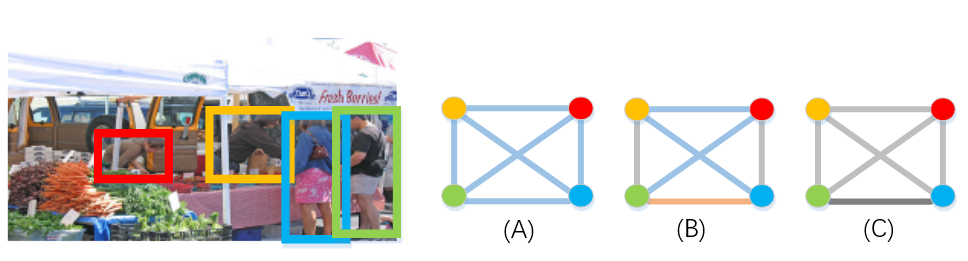
\includegraphics[width=0.90 \textwidth,clip]{case-2.png}
    	%\hspace{0.02\textwidth}
    	%\vspace*{-0.08cm}
        %\caption{数据集的关系类别统计}
    	\vspace*{-3.3mm}
    }
    \subfigure[]{
    	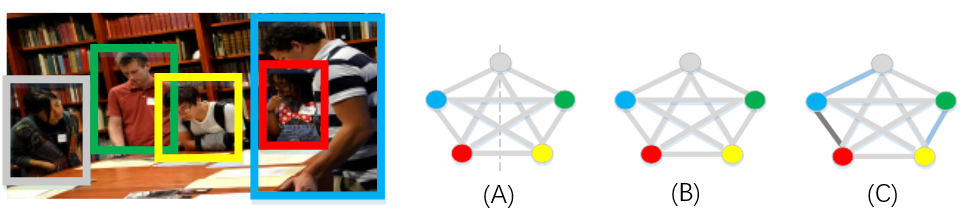
\includegraphics[width=0.90 \textwidth,clip]{case-3.png}
    	%\hspace{0.02\textwidth}
    	%\vspace*{-0.08cm}
        %\caption{数据集的关系类别统计}
    	\vspace*{-2.5mm}
    }
    \subfigure[]{
    	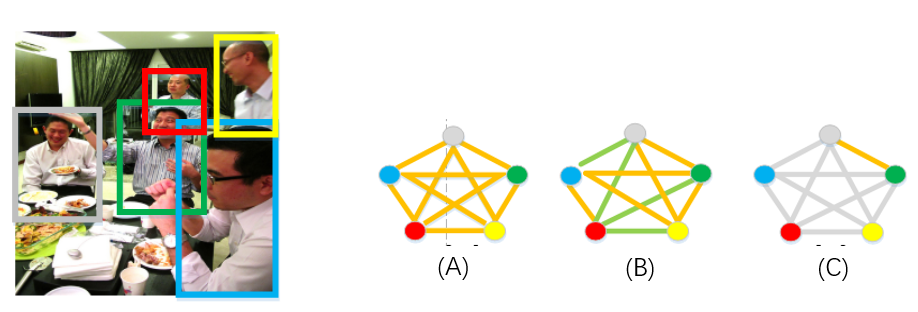
\includegraphics[width=0.90 \textwidth,clip]{case-4.png}
    	%\hspace{0.02\textwidth}
    	%\vspace*{-0.08cm}
        %\caption{数据集的关系类别统计}
    	\vspace*{-2.5mm}
    }
     \subfigure{
    	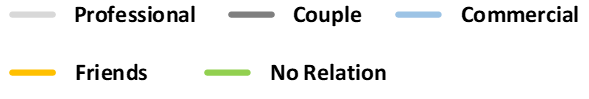
\includegraphics[width=0.80 \textwidth,clip]{case-color.png}
    	%\hspace{0.02\textwidth}
    	%\vspace*{-0.08cm}
        %\caption{数据集的关系类别统计}
    	\vspace*{-2.5mm}
    }
    \caption{PISC-fine数据集中,PPRN表现比GRM模型好的部分测试样本}
    \label{fig:exp-case-study}
\end{figure}

\section{本章小结}

本章节主要介绍和分析了PPRN模型在PISC和PIPA-relation两个社会关系理解数据集上的实验结果。

首先,本章介绍了两个大型数据集的图片来源、构造方式、关系类别的划分,其中PISC数据集包含两种关系粒度,PIPA-relation包含5个关系域和这5个关系域对应的15种关系类别。与此同时,本文统计了各检测个数据集划分的图片数量,人对数量。本章进一步分析数据集的特点,具体来说包括两个指标:包含多个人对的图片比例,以及包含多种关系类别的比例。同时,本章给出了实验结果的评价方法mAP,并且举例说明了在物体识别领域怎么计算mAP。接着,本章给出了模型的参数设置、不同训练步骤的优化方法。

然后,我们分别在这两个数据集上进行了社会关系检测这项社会关系理解任务,给出了对比实验组的设定,详细说明了对比工作引入了哪些信息、有哪些设定。在实验结果中,我们分别给出了每个关系类别的的召回率和测试集上的mAP。从实验结果来看,融合关系上下文的模型,结合同一图像中其它关系的约束能提高关系的表达能力,在PISC-fine和PIPA-relation的实验结果超过了设置的对照组。接着,本章对消息池化模块采用了不同的池化方法进行对比,发现现有的池化方法超过了常见的平均池化和最大池化。另外,在消息传递机制之后,本章实现了一个结合周边物体信息模块,发现这部分的信息加入后并没有进一步提高实验结果。通过之后的分析,本文发现不管是引入周边物体的信息还是先验知识,均属于场景信息,但是这部分的信息可以由当前图片中其它人对的关系提供,并且不存在额外的检测标注、噪声引入。

最后,本章进行了案例分析,给出了一些真实测例的结果。


